%!TEX root = ../../PhD_thesis__Edouard_Leurent.tex
\graphicspath{{3-Appendices/1-Appendix/}}

\chapter{The \textsc{highway-env} software}

\minitocStartChapterNoNewPage{}

\label{chapter:a}

\section{General presentation}

\textsc{highway-env} is a collection of environments for behavioural planning tasks in autonomous driving.

Each environment specifies a full \gls{MDP} to describe a particular decision-making problem that an autonomous vehicle may face.

\paragraph{Origins}
When I started my Ph.D., there existed more ambitious open-source simulators that relied on heavy physics engines and 3D graphics, such as TORCS \citep{Wymann15torcs:the}, Airsim \citep{shah2017airsim} and CARLA \citep{Dosovitskiy2017}. However, those were better suited for low-level sensing and control, \eg training of visuomotor policies in a single-agent setting. On the other hand of the spectrum, SUMO \citep{SUMO2018} was rather meant for high-scale traffic optimisation and lacked details and flexibility on local dynamics. In contrast, I needed a simulator focused on high-level decisions and vehicle-to-vehicle interactions. Consequently, I launched \textsc{highway-env} with the intent of having a minimalist simulator, implemented fully in Python for fast prototyping and easy interfacing with \gls{RL} libraries.

\paragraph{Usage}
We show below a basic use of \textsc{highway-env}, with a code snipped showing the interaction between the environment, which generates observations and rewards, and the agent which provides actions according to its policy.

\begin{lstlisting}[language=Python,frame=single,caption={Create, step and render the \texttt{highway-v0} environment.},captionpos=b]
import gym
import highway_env

env = gym.make('highway-v0')

done = False
while not done:
    action = ... # Your agent code here
    obs, reward, done, info = env.step(action)
    env.render()
\end{lstlisting}

\paragraph{The environments}

To this day, \textsc{highway-env} comes with six different scenes, configured with suitable observation space $\cS$, action space $\cA$ and reward function $\reward$, illustrated in \Cref{tab:environments}.

\begin{table}[ht]
	\begin{tabular}{cc}
		\begin{subfigure}{0.49\textwidth}\centering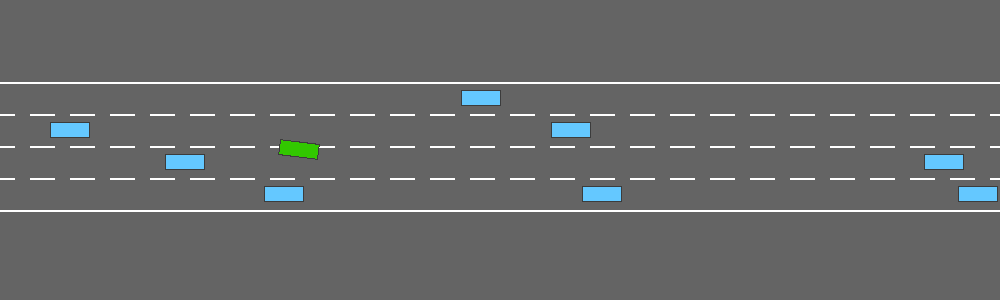
\includegraphics[width=\columnwidth]{img/highway}\caption{Highway}\end{subfigure}&
		\begin{subfigure}{0.49\textwidth}\centering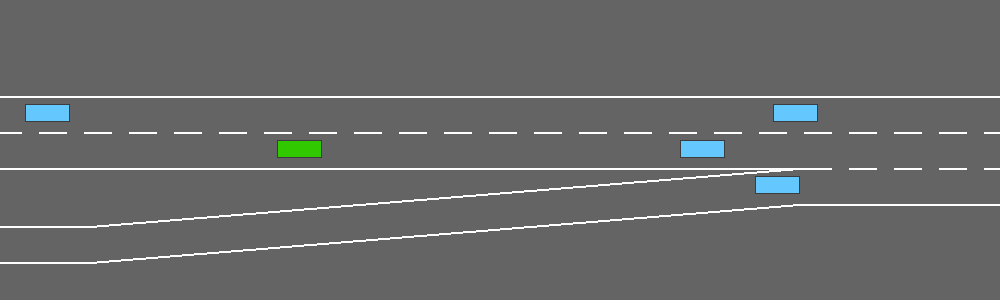
\includegraphics[width=\columnwidth]{img/merge}\caption{Merge}\end{subfigure}\\
		\newline
		\begin{subfigure}{0.49\textwidth}\centering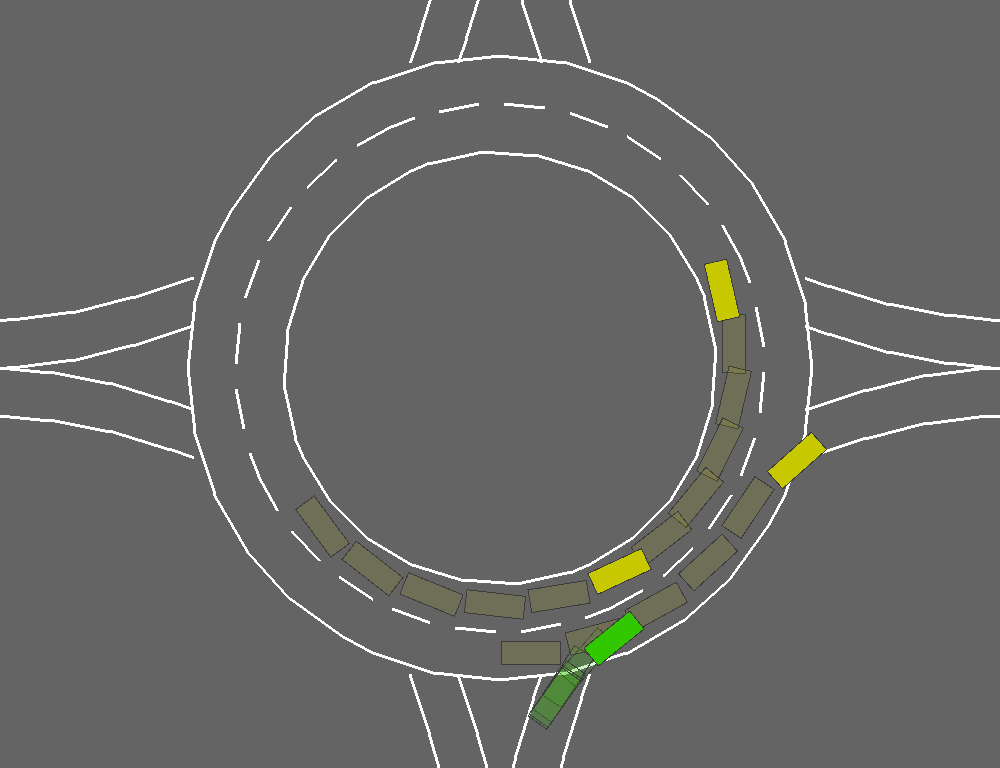
\includegraphics[width=\columnwidth]{img/roundabout}\caption{Roundabout}\end{subfigure}&
		\begin{subfigure}{0.49\textwidth}\centering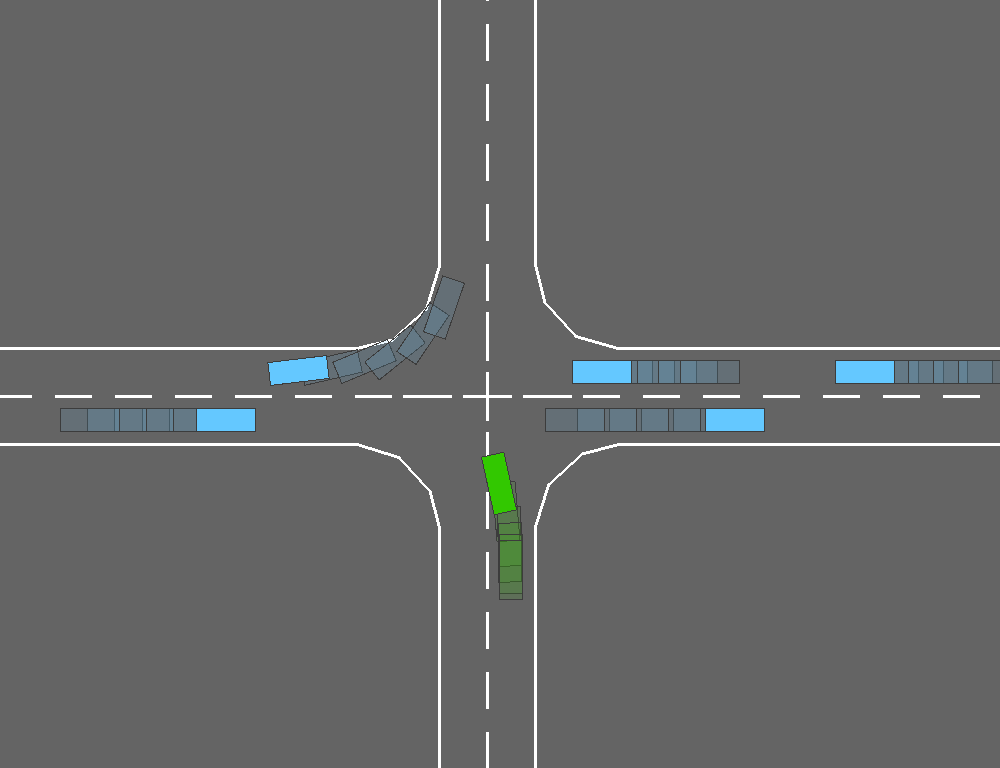
\includegraphics[width=\columnwidth]{img/intersection}\caption{Intersection}\end{subfigure}\\
		\begin{subfigure}{0.49\textwidth}\centering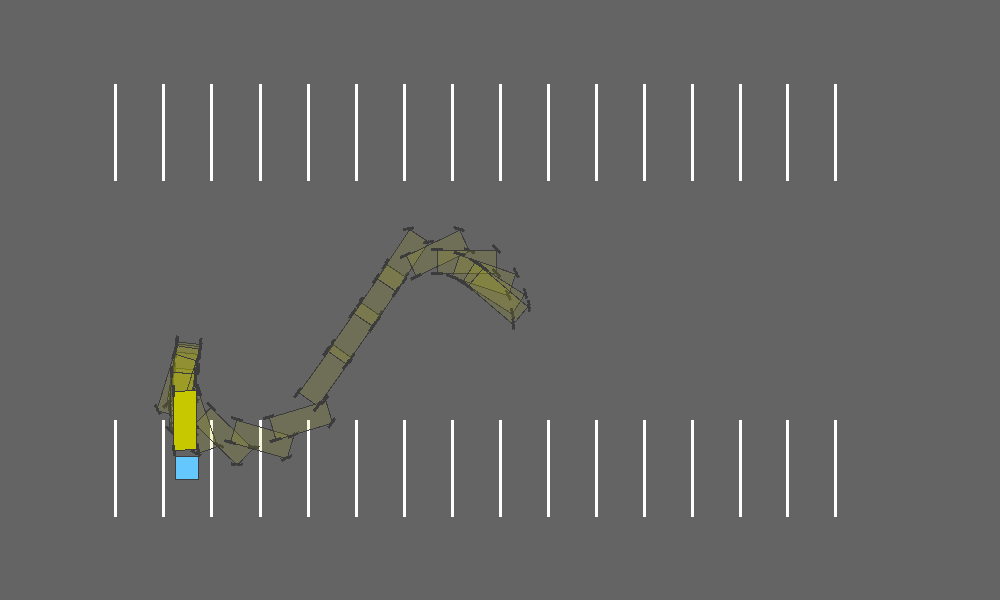
\includegraphics[width=\columnwidth]{img/parking}\caption{Parking}\end{subfigure}&
		\begin{subfigure}{0.49\textwidth}\centering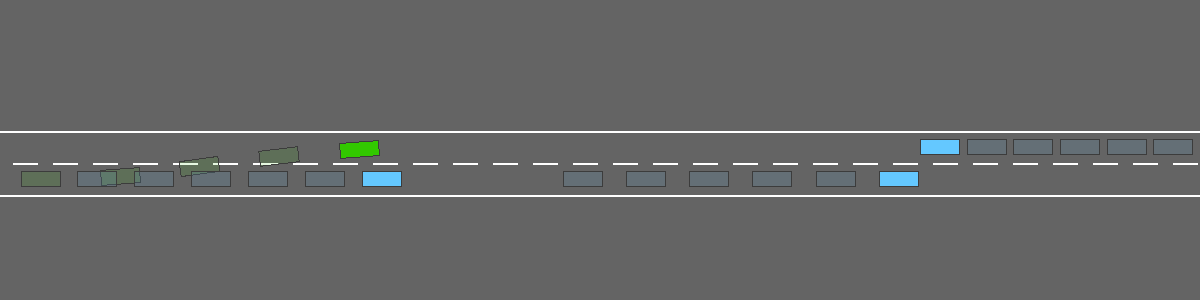
\includegraphics[width=\columnwidth]{img/two-way}\caption{Two-way}\end{subfigure}\\
	\end{tabular}
	\caption{The different environments available in \textsc{highway-env}.}
	\label{tab:environments}
\end{table}

\begin{itemize}
	\item \textbf{Highway.} The vehicle is driving on a highway populated with other drivers. The goal is to drive as fast as possible while avoiding collisions with other vehicles, through a discrete meta-action space of manoeuvres.
	\item \textbf{Merge.} The task is similar to \texttt{highway-v0}, but a vehicle is incoming from an access ramp and must be able to merge successfully in traffic. To that end, the ego-vehicle must change lane or adapt its velocity so that the merging vehicle has sufficient space. This task is inspired by a practical use case for \gls{ADAS} systems at Renault.
	\item \textbf{Roundabout.} The vehicle must cross a roundabout as fast as possible while avoiding collisions. It requires reasoning about the uncertain destinations of other vehicles.
	\item \textbf{Intersection.} This environment is similar to roundabout, but with an increased density of vehicles and types of conflicts. Only the throttle is controlled, and the steering is performed automatically to track the ego-vehicle destination.
	\item \textbf{Parking.} A goal-conditioned continuous control environment: the desired parking spot location is part of the observation, and the ego-vehicle must plan cusp-shaped manoeuvres to reach it with the proper heading.
	\item \textbf{Two-way.} This environment is similar to highway, except that the ego-vehicle can change to a lane facing the opposite direction, with incoming vehicles. This enables to highlight an efficiency-safety trade-off for risk-sensitive decision-making.
\end{itemize}

\paragraph{Features}

Several parts of the environment can be configured.

\begin{itemize}
	\item \textbf{Observations.} Several types of observations are available, such as the \emph{list of features} and \emph{occupancy grid} described in \Cref{chapter:4}. Other types include RGB images, time-to-collision maps, and goal locations.
	\item \textbf{Actions.} In addition to the discrete meta-action space $\cA$ described in \Cref{chapter:3}, a continuous space $\cA=\Real^2$ for throttle and steering can also be selected.
	\item \textbf{Dynamics.} Other vehicles can follow the \gls{IDM} and \gls{MOBIL} behavioural models as described in  \Cref{chapter:3} or its linearised version of \Cref{sec:prediction}. The ego-vehicle can be controlled with either the Kinematic Bicycle Model as in \Cref{chapter:3} or the Dynamic Bicycle Model as in  \Cref{sec:robust-stabilisation}.
	\item \textbf{Rewards.} The rewards and penalties associated with speed or collisions are configurable.
	\item \textbf{Graphics.} Graphics are rendered using the \href{https://www.pygame.org/news}{pygame} library, window size and resolution can be configured.
\end{itemize} 


\paragraph{Development process}

The project closely follows the insights of \Cref{chapter:3} in its definition of the traffic state, actions, dynamics, and rewards. See the \href{https://highway-env.readthedocs.io/en/latest/user\_guide.html}{user guide} in the documentation for more details.

It also complies by the \href{https://github.com/openai/gym}{OpenAI gym} standard interface for \gls{RL} environments. Continuous integration (CI) is performed with \href{https://docs.pytest.org/en/stable/}{pytest} unit tests automatically triggered with \href{https://github.com/features/actions}{GitHub actions}. The documentation is built from the source code comments using \href{https://www.sphinx-doc.org/en/master/}{Sphinx}, and hosted on \href{https://readthedocs.org/}{Read the Docs}. Finally, multiple examples can be run directly from the browser through \href{https://colab.research.google.com/}{Google Colab} notebooks.

\section{Outreach}
\label{sec:outreach}
In this section, we document the dissemination of the library among several communities.

\subsection{Academia}

We highlight that several researchers have reported using \textsc{highway-env} in their publications and submissions:
\begin{itemize}
	\item \fullcite{Li2019}
	\item \fullcite{Yang2020}
	\item \fullcite{n2020smart}
	\item \fullcite{Xu2020taskagnostic}
	\item \fullcite{ma2020dsac}
	\item \fullcite{mei2020prioritized}
\end{itemize}

\leavevmode\newline
Additionally, we use it in most of our own publications:
\begin{itemize}
	\item \fullcite{Leurent2018approximate}
	\item \fullcite{Leurent2019interval}
	\item \fullcite{Leurent2019social}
	\item \fullcite{CarraraLeurent2019}
	\item \fullcite{Leurent2020practical}
	\item \fullcite{Leurent2020robust}
	\item \fullcite{Leurent2020beyond}
\end{itemize}

%Mohammad Hussein Tavakoli Bina, Department of Electrical Engineering, Amirkabir University of Technology, see \href{https://github.com/mhtb32/tl-env}{tl-env}
\leavevmode\newline
\noindent Finally, the \textsc{highway-env} library is featured in the documentation and examples of two of the most famous libraries in the \gls{RL} ecosystem:
\begin{itemize}
\item \href{https://github.com/openai/gym}{OpenAI Gym}, a standard interface for comparing \gls{RL} algorithms. \textsc{highway-env} is mentioned in the \href{https://github.com/openai/gym/blob/master/docs/environments.md#highway-env-tactical-decision-making-for-autonomous-driving}{list of environments}.
\item \href{https://github.com/hill-a/stable-baselines}{Stable Baselines}, a set of improved implementations of \gls{RL} algorithms based on OpenAI Baselines. \textsc{highway-env} is used as an  \href{https://stable-baselines.readthedocs.io/en/master/guide/examples.html#hindsight-experience-replay-her}{example} in the documentation.
\end{itemize}

\subsection{Education}

Since the publication of \textsc{highway-env}, many masters students have contacted me throughout the years, and reported using the simulator for their final project of in various courses, occasionally upon suggestion by their professor. %Ayaz Samadli
I did not keep track of all these exchanges, but as a trace of this activity, see:
\begin{itemize}
	\item the \href{https://github.com/eleurent/highway-env/issues?q=is\%3Aissue}{list of issues} opened in \textsc{highway-env}.
	\item the \href{https://github.com/eleurent/rl-agents/issues?q=is\%3Aissue}{list of issues} opened in \textsc{rl-agents}.
\end{itemize} 

\subsection{Industry}

Several engineers, mainly from the Automotive industry, have demonstrated interest in \textsc{highway-env}, either by reaching out to me directly or by developing their own project on top of the library. To name a few,

\begin{itemize}
    \item \href{https://www.linkedin.com/in/simon-chauvin/}{Simon Chauvin}, Machine Learning Engineer at Autonomous Driving at \href{https://www.esrlabs.com/}{ESR Labs AG}, who contacted me to reproduce my results.
	\item \href{https://www.linkedin.com/in/huberclement}{Clément Huber}, Product Owner in the Path Planning team at \href{https://navya.tech/fr/}{NAVYA Group}, and \href{https://www.linkedin.com/in/lucas-boyer}{Lucas Boyer}, intern in that team, contacted me on several occasions to discuss the \href{https://github.com/lucasBOYER/highway-env}{internship} of Lucas based on \textsc{highway-env} and \textsc{openai/baselines}.
	\item \href{https://www.linkedin.com/in/munirjojoverge}{Munir Jojo-Verge}, Motion Planning and Decision Making Manager at \href{https://canvas.technology/}{Amazon Robotics}, who wrote to me regarding his extension of \textsc{highway-env} to continuous actions, see \href{https://github.com/munirjojoverge/rl_AD_urban_baselines}{his fork} which lead to the addition of the \texttt{parking-v0} environment.
	\item \href{https://www.linkedin.com/in/deepdrive}{Craig Quiter}, Founder of \href{https://deepdrive.voyage.auto/}{Deepdrive} at \href{https://voyage.auto/}{Voyage}, who mentioned that \href{https://medium.com/@crizcraig/smooth-operator-92c6c14862fb}{his recent work} was inspired by \textsc{highway-env} and with whom I had the pleasure to discuss.
	\item \href{https://www.linkedin.com/in/pinaki-gupta/}{Pinaki Gupta}, Behaviour Planning architect at \href{https://lucidmotors.com/}{Lucid Motors}, see \href{https://github.com/pinakigupta/BehaviorRL}{his fork} that features variants of the \texttt{two-way-v0} and \texttt{parking-v0} environments augmented with additional vehicles and multiple goals.
	\item \href{https://www.linkedin.com/in/guillaumealleon}{Guillaume Alleon}, Head of AI research at \href{https://www.airbus.com/}{Airbus}, see \href{https://github.com/galleon/highway-env}{his fork}.
    \item \href{https://ru.linkedin.com/in/boris-yangel-83194729}{Boris Yangel}, Principal Software Engineer at \href{https://yandex.com/}{Yandex}, see \href{https://github.com/hr0nix/trackdays/blob/master/setup.py}{his project}.
\end{itemize}


 


